\documentclass[tikz,border=0cm,dvipsnames,x11names,rgb]{standalone}

\usepackage{amsmath,amssymb,amsfonts}
\usetikzlibrary{calc,
fit,
shapes.misc,
shapes.geometric,
arrows.meta,
fadings,
matrix,
chains,
scopes,
positioning}

\usepackage{pgfplots}
\usepackage{pgfplotstable}
\pgfplotsset{compat=1.18}



\usepackage[]{fontspec}

\setmainfont{Latin Modern Roman}
\setmonofont{Latin Modern Math}
\renewcommand{\textsc}[1]{{\fontfamily{lmr}\selectfont \scshape #1}}

\usepackage[]{bm}

\makeatletter
\@ifundefined{fromRoot}{\newcommand{\fromRoot}[1]{../../#1}}{}

\def\input@path{{../..}{..}{.}{./svg}{./pgfplots}{./tikzpicture}}
%or: \def\input@path{{/path/to/folder/}{/path/to/other/folder/}}
\makeatother

\newcommand*{\gf}[1]{\acrshort{gf}($#1$)}%
\newcommand*{\mpn}[1]{\bm{P}_{#1}}%
\newcommand*{\pn}[1]{%
  \ifthenelse{\equal{#1}{}}{$\mpn{0}$}{$\mpn{#1}$}%
}%

\newcommand*{\pk}[3]{%
  \ifthenelse{\equal{#1}{#2}}{\textcolor{red}{\phantom{.}$p_0$\phantom{.}}}{\phantom{.}$p_#3$\phantom{.}}%
}%


\newcommand*{\placeholder}{
\includegraphics[width=\linewidth, height=.25\textheight, keepaspectratio = true]{figures/certified_xilinx.png}}%

\newcommand*{\snr}{\acrshort{snr}}%
\newcommand*{\snrs}{\acrshortpl{snr}}%

\newcommand*{\mpd}[0]{p_\Delta}%
\newcommand*{\mpo}[0]{p_\omega}%
\newcommand*{\pd}[0]{$\mpd$}%
\newcommand*{\po}[0]{$\mpo$}%
\newcommand*{\mpfa}[0]{\mathcal{P}_{fa}}%
\newcommand*{\mpmd}[0]{\mathcal{P}_{md}}%
\newcommand*{\pfa}[0]{\acrshort{pfa}}%
\newcommand*{\pmd}[0]{\acrshort{pmd}}%
\newcommand*{\mnorm}[1]{\mathcal{L}_{#1}}%
\newcommand*{\norm}[1]{$\mnorm{#1}$}%
\newcommand*{\fft}{\acrshort{fft}}%
\newcommand*{\mfft}[1]{\mathcal{F}(#1)}%
\newcommand*{\mifft}[1]{\mathcal{F}^{-1}(#1)}%
\newcommand*{\ts}{\acrshort{ts}}%

\newcommand*{\cpp}[1]{C\textrm{++#1}}%
\newcommand*{\na}{\textrm{\textcolor{SlateGray4}{N/A}}}%

\newcommand*{\vect}[1]{\bm{#1}}%
\newcommand*{\mat}[1]{\bm{\mathrm{#1}}}%

\newcommand*{\task}[1]{\mathcal{T}_{#1}}%

\newcommand*{\sdr}{\acrshort{sdr}}%
\newcommand*{\fpga}{\acrshort{fpga}}%



\begin{document}

\begin{tikzpicture}[very thick, inner sep = 1 mm]

  \node [
    anchor = north east
  ] (bat) at (0,0){\texttt{Power Grid}};
  \node [
    align=center,
    anchor = north
  ] (pi4) at ($(bat.south) + (0, -1)$) {\texttt{Linux}\\\texttt{Laptop}};
  \node [
    align = center,
    anchor = east
  ] (usrp) at ($(pi4.west) + (-3, 0)$) {\texttt{USRP}\\\texttt{X310}};


  \draw [-Triangle] (bat.south) -> (pi4.north)
  node [midway, left, font={\scriptsize}] {\textit{power}};
  \draw [-Triangle] (bat.west) -| (usrp.north)
  node [pos=.8, right, font={\scriptsize}] {\textit{power}};
  \draw [Triangle-] (pi4.west) -> (usrp.east)
  node [midway, above, font={\scriptsize}] (stream) {\textit{sample stream}};
  \node [anchor=north, font={\scriptsize}] at (stream.south) {$500$ \textit{ks/s}};

  \coordinate (ant_usrp) at ($(usrp.west) + (-1,0)$);
  \draw [Triangle-] (usrp.west) -- (ant_usrp);
  \draw (ant_usrp) -- ($(ant_usrp) + (0, .75)$);
  \draw ($(ant_usrp) + (0, .75)$) -- ($(ant_usrp) + (+.25, 1)$);
  \draw ($(ant_usrp) + (0, .75)$) -- ($(ant_usrp) + (   0, 1)$);
  \draw ($(ant_usrp) + (0, .75)$) -- ($(ant_usrp) + (-.25, 1)$)
  node[ pos = 1, anchor = south west, font={\tiny}] {$433.92$ \textit{MHz}};

  \node [] (ant) at (ant_usrp) {};

  \node [
    draw,
    dashed,
    inner sep = 4mm,
    % label=below:Building (\textit{ENSIBS}) roof,
    fit = (bat) (pi4) (ant) (bat)
  ] (v) {};

  \node [left = 1 mm of v, inner sep = 0pt]  {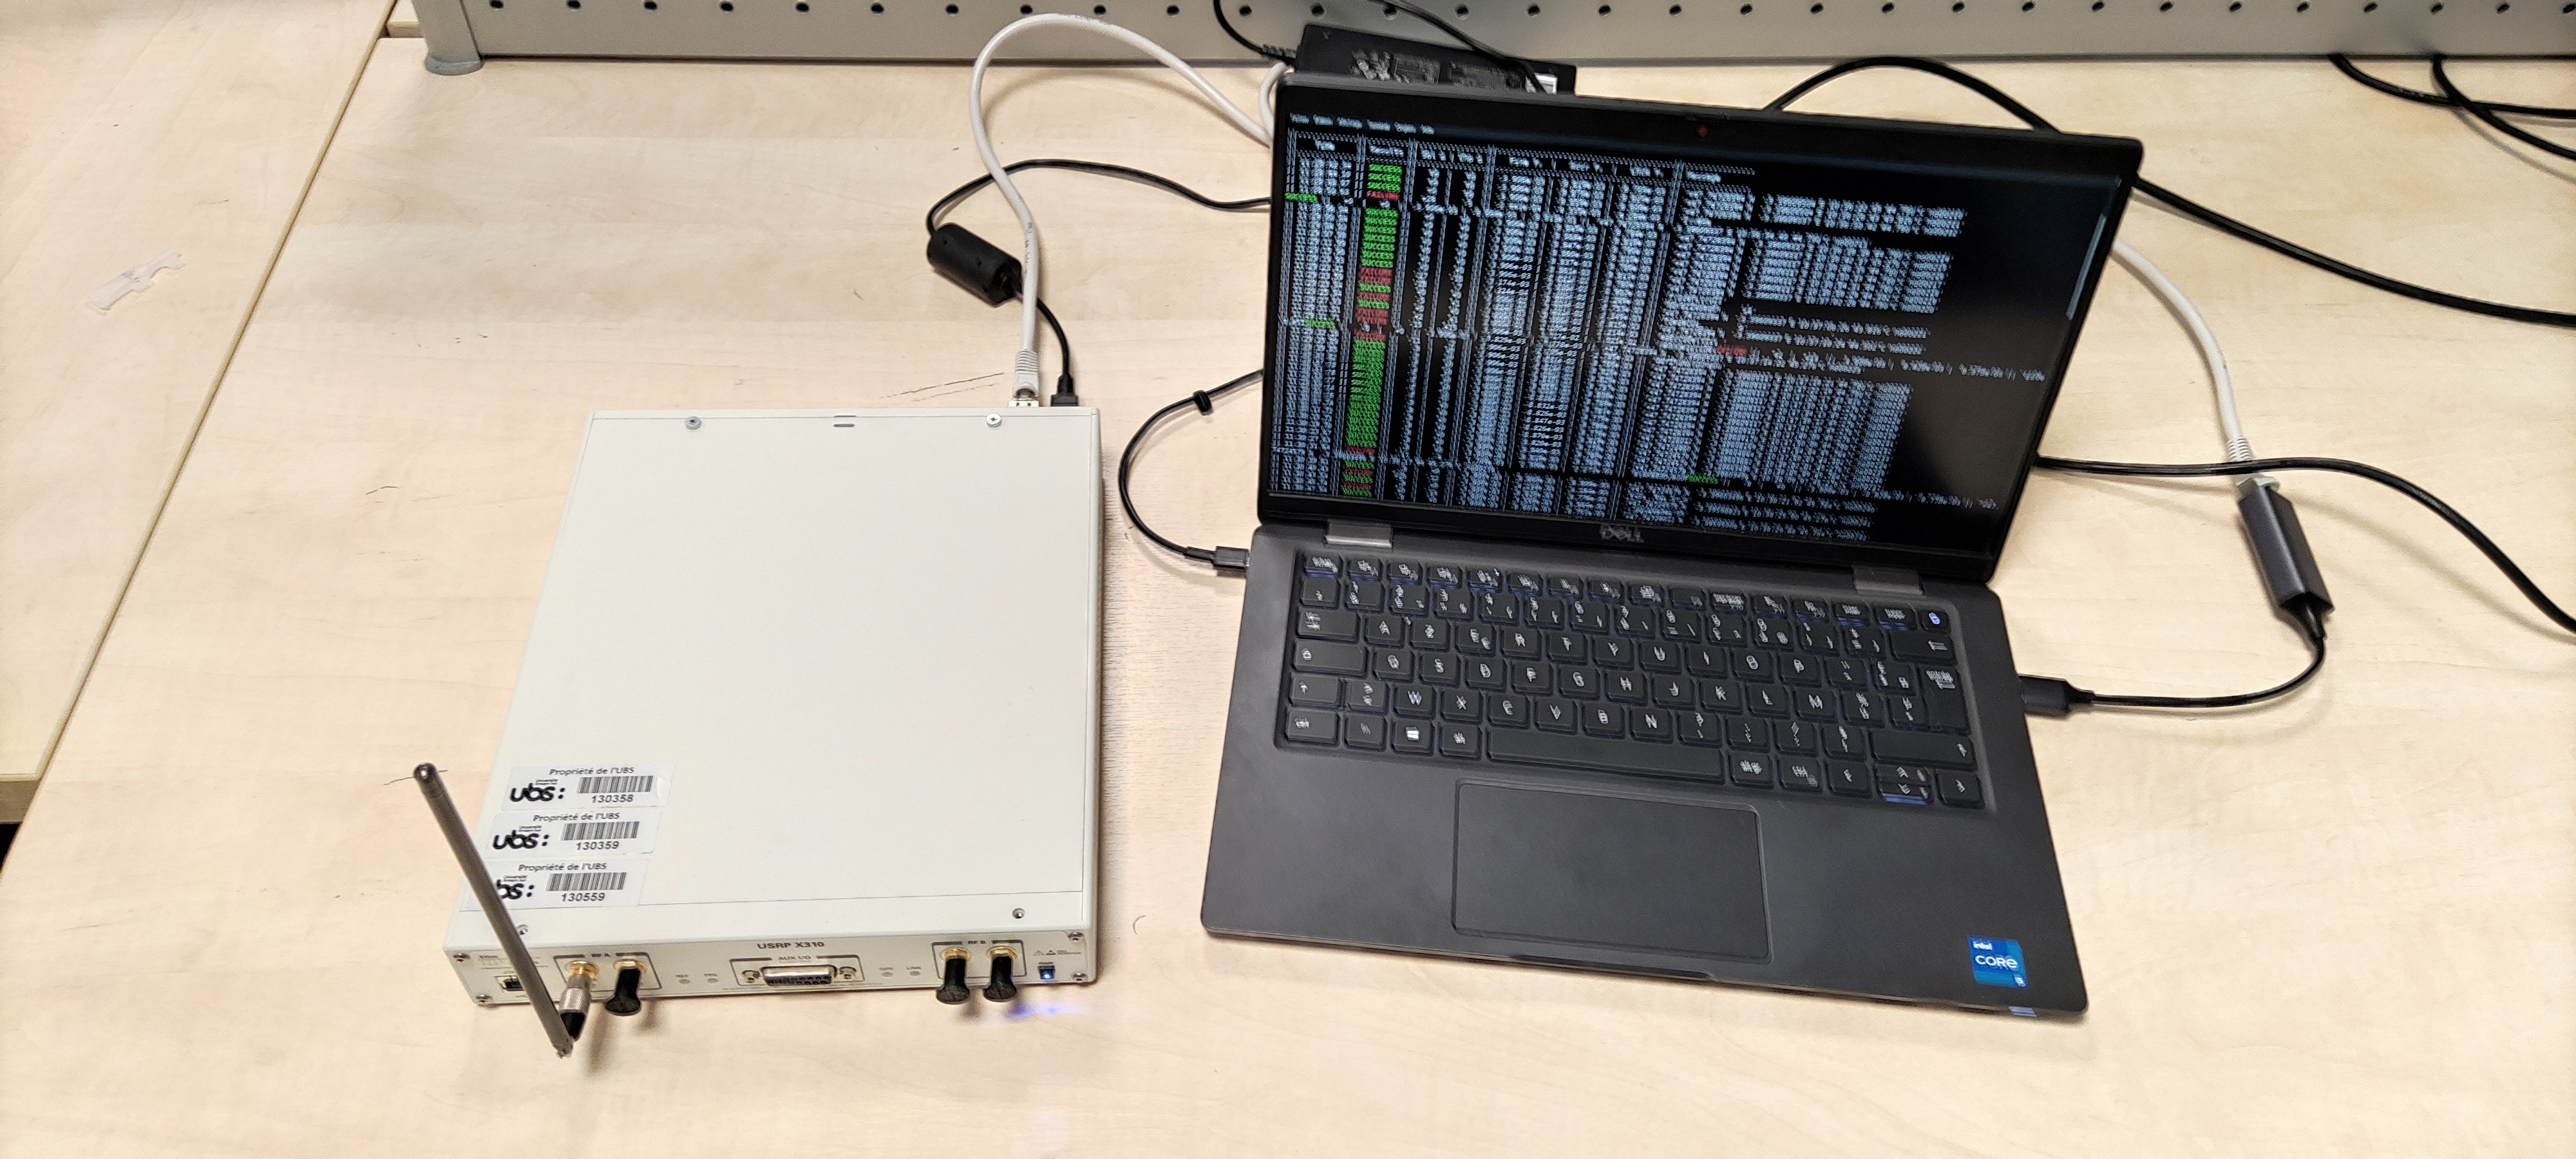
\includegraphics[width = 5.5 cm, clip, trim = {20cm 5cm 23cm 3.5cm}]{\fromRoot{figures/rtexps-pics/IMG_20221027_180621.jpg}}};
  \node[dashed, draw=red, fit={(-12.9, -0.75) (-10.8, -2.65)}] {USRP};
  \node[dashed, draw=RoyalBlue, label={above:Laptop}, fit={(-10.45, -2.65) (-7.65, .2)}] {};

  \node [right = 1 mm of v, inner sep = 0pt] (rcvs)  {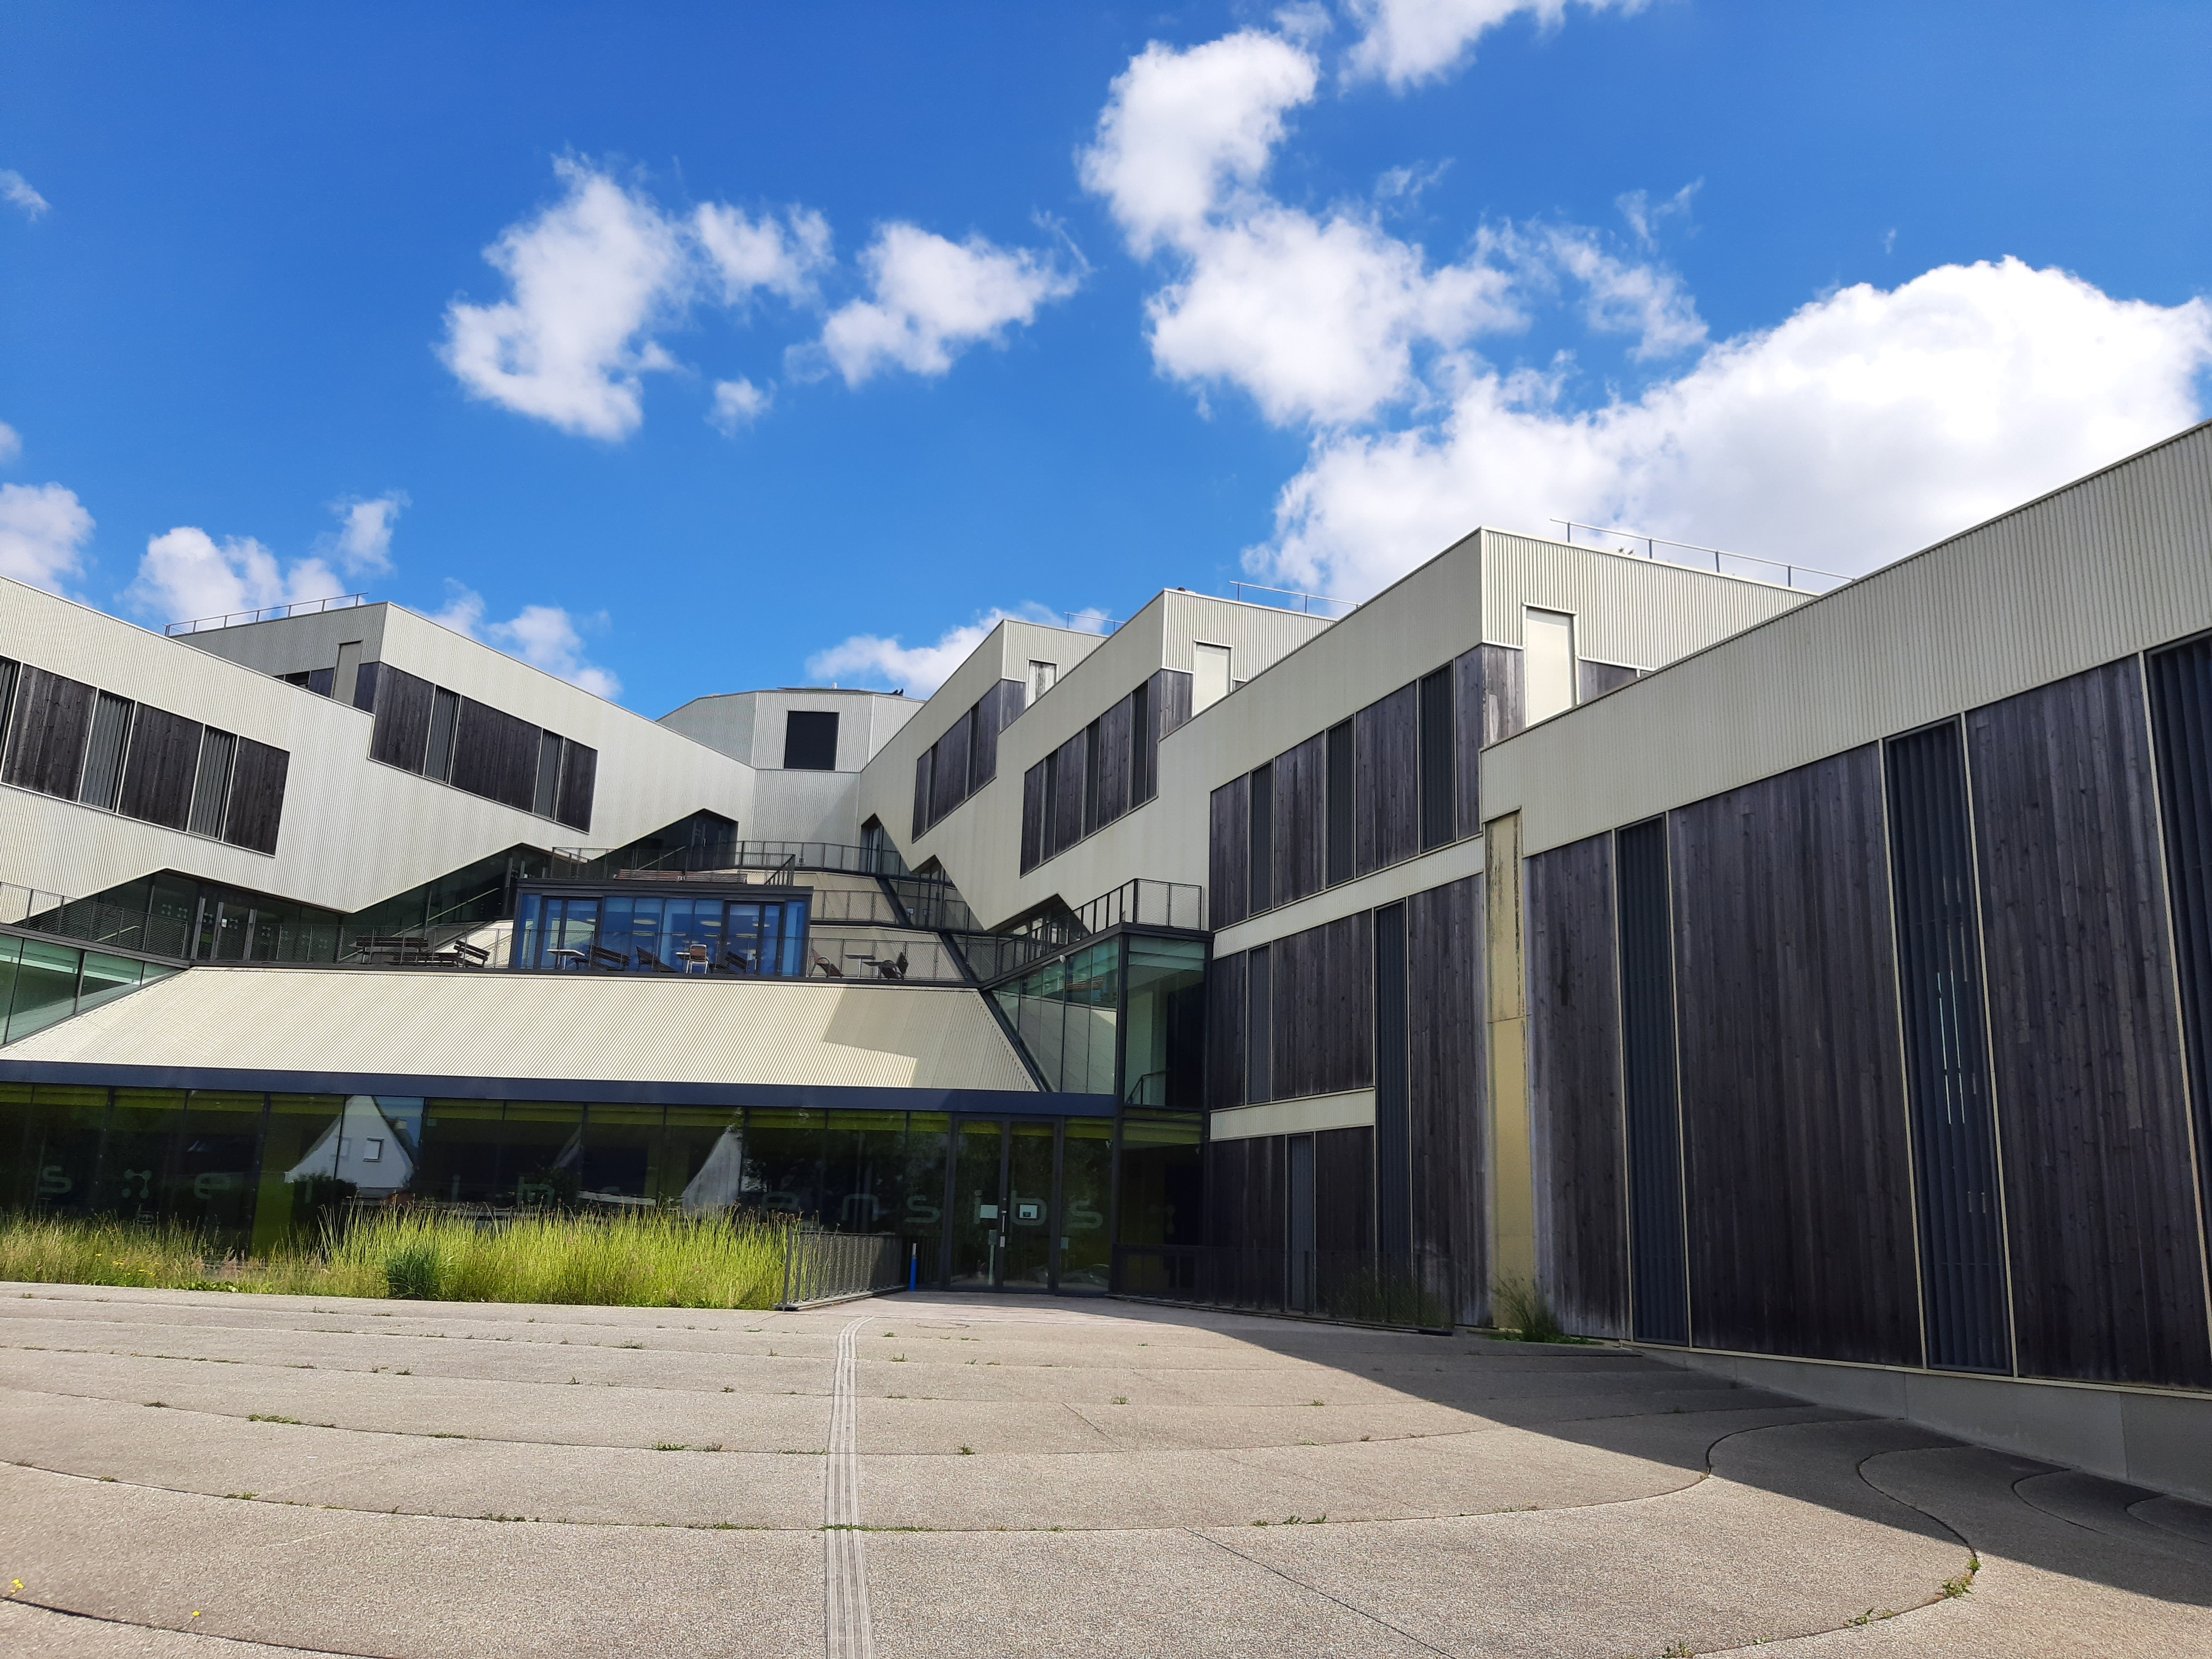
\includegraphics[width = 3 cm]{\fromRoot{figures/rtexps-pics/receiver_spot.jpg}}};
  \draw [red, ->] (rcvs.north) -- ($(rcvs.north) + (0, -.8)$)
  node [pos = 0, above] {\textbf{Here}};
\end{tikzpicture}
\end{document}
